\documentclass[diplomskirad]{fer}
% Dodaj opciju upload za generiranje konačne verzije koja se učitava na FERWeb
% Add the option upload to generate the final version which is uploaded to FERWeb

\usepackage{bm}

%--- PODACI O RADU / THESIS INFORMATION ----------------------------------------

% Naslov na hrvatskom jeziku / Title in Croatian
\naslov{Varijacijsko učenje na zašumljenim oznakama}

% Broj rada / Thesis number
\brojrada{872}

% Autor / Author
\author{Dominik Jambrović}

% Mentor 
\mentor{prof.\ dr.\ sc.\ Siniša Šegvić}

% Datum rada na hrvatskom jeziku / Date in Croatian
\datum{lipanj, 2025.}

%-------------------------------------------------------------------------------


\begin{document}


% Naslovnica se automatski generira / Titlepage is automatically generated
\maketitle


%--- ZADATAK / THESIS ASSIGNMENT -----------------------------------------------

% Zadatak se ubacuje iz vanjske datoteke / Thesis assignment is included from external file
% Upiši ime PDF datoteke preuzete s FERWeb-a / Enter the filename of the PDF downloaded from FERWeb
\zadatak{hr_0036534818_94.pdf}


%--- ZAHVALE / ACKNOWLEDGMENT --------------------------------------------------

\begin{zahvale}
  % Ovdje upišite zahvale / Write in the acknowledgment
  Zahvale!
\end{zahvale}


% Odovud započinje numeriranje stranica / Page numbering starts from here
\mainmatter


% Sadržaj se automatski generira / Table of contents is automatically generated
\tableofcontents


%--- UVOD / INTRODUCTION -------------------------------------------------------
\chapter{Uvod}
\label{pog:uvod}
  
Duboki modeli koriste se u brojnim aspektima naše svakodnevice.\ Pri razvoju i učenju modela, pažnju prije svega posvećujemo performansama na neviđenim podatcima - želimo naučiti modele koji dobro generaliziraju.\ 
Drugim riječima, želimo da modeli daju ispravna predviđanja za viđene, ali i za neviđene podatke.\ Ovime osiguravamo da naša rješenja imaju primjenu i van laboratorijskih uvjeta u kojima se uče.\
  
U procesu razvoja modela za određeni zadatak strojnog učenja, osim odabira arhitekture, algoritma učenja i hiperparametara, veliku ulogu igraju podatci na kojima učimo.\ 
Općenito govoreći, prikupljanje i označavanje podataka jedan je od najskupljih dijelova procesa razvoja rješenja za nekih problem.\ 
Važno je da prikupljeni podatci što realističnije predstavljaju stvarne situacije s kojima će se naš model susretati tj.\ da distribucija podataka odgovara stvarnoj distribuciji situacija koje prikazuju.\ 
Dodatno, pokazuje se da duboki modeli uz dovoljan kapacitet mogu naučiti ispravno predviđati oznake čak i za nasumično označene podatke~\cite{zhang2016understanding}, tako da je veoma važno da su prikupljeni podatci što točnije označeni.\
  
Područje računalnog vida~\cite{voulodimos2018deep} bavi se razvojem algoritama i modela za brojne zadatke raspoznavanja i razumijevanja slika.\ Najčešći zadatak je klasifikacija slika - model na ulazu dobiva sliku, a na izlazu treba predvidjeti razred koji odgovara ulaznom primjeru.\ 
Iako postoje brojni skupovi slikovnih podataka koji se mogu koristiti za učenje i evaluaciju modela, za konkretne zadatke u većini slučajeva trebamo prikupiti i označiti vlastite slike.\ 
Pritom postoji nekoliko čestih opasnosti: prisutnost zatrovanih podataka~\cite{biggio2012poisoning} ili zašumljenih oznaka~\cite{gupta2019dealing}.\ 

\pagebreak

Kada govorimo o trovanju podataka, maliciozni agent u skup podataka dodaje zatrovane podatke s ciljem manipulacije izlaza naučenog modela za određene ulaze.\ 
S druge strane, anotator podataka bez zlih namjera određenim podatcima može pridijeliti netočne oznake, time dodajući podatke sa zašumljenim oznakama u skup.\ 
Kroz vrijeme, razvili su se brojni algoritmi za obranu modela od zatrovanih podataka~\cite{li2021anti, huang2022backdoor, gao2023backdoor}, kao i za učenje na zašumljenim oznakama~\cite{liu2022robust, chen2024imprecise}.\ Ipak, većina radova se fokusira na samo jedan od ovih problema, a ne na razvoj algoritma koji se može nositi s oba problema.\ 
  
Cilj ovog rada je reproducirati i poboljšati rezultate okvira za obranu od zatrovanih podataka imena VIBE (engl.\ \textit{Variational inference for backdoor elimination})~\cite{sabolic2025seal}.\ 
Osim ovoga, cilj je i primijeniti VIBE na problem zašumljenih oznaka.\ Pritom VIBE evaluiramo na nekoliko čestih vrsta trovanja odnosno zašumljivanja oznaka kako bi se osigurala robusnost okvira.\ 
Dodatno, cilj je usporediti VIBE sa stanjem tehnike (engl.\ \textit{state of the art - SotA}) za problem zašumljenih oznaka.\
%-------------------------------------------------------------------------------
\chapter{Problem zatrovanih podataka}
\label{pog:zatrovani}

Cilj dodavanja zatrovanih podataka~\cite{biggio2012poisoning} u skup je ugrađivanje stražnjih vrata (engl.\ \textit{backdoor}) u naučeni model.\ Ako napad uspije, napadač može kontrolirati izlaz modela koristeći suptilne izmjene ulaznog primjera.\ 
Općenito govoreći, stvaranje zatrovanih podataka podrazumijeva dodavanje vizualnog okidača na ulazni primjer, kao i prikladnu izmjenu oznaka.\ Pritom napadač radi izmjenu određenog udjela podataka, dok preostali podatci ostaju neizmjenjeni.\ 
Hiperparametar koji opisuje udio zatrovanih podataka zvat ćemo stopom trovanja (engl. \textit{poisoning rate}).\ Pojedine metode trovanja podataka razlikuju se po načinu dodavanja okidača tj.\ načinu izmjene ulaznih primjera, kao i po načinu izmjene oznaka.\ 
  
Kada govorimo o načinu izmjene ulaznih primjera, možemo napraviti podjelu na lokalne i globalne izmjene primjera.\ Kod lokalnih izmjena, mijenja se samo određeno područje slike, najčešće dodavanjem zadanog okidača na to područje~\cite{gu2019badnets}.\ 
S druge strane, kod globalnih izmjena se mijenja cijela slika koristeći različite tehnike poput miješanja slike s okidačem~\cite{chen2020backdoor} ili transformiranja slike na temelju zadanog deformacijskog polja~\cite{nguyen2021wanet}.\ 
Osim korištenja jednog okidača za sve zatrovane podatke, određeni napadi koriste okidače specifične za pojedini uzorak~\cite{li2021invisible}.\
  
Većinu napada možemo svrstati u jedan od dva načina izmjena oznaka: \textit{all-to-one} i \textit{all-to-all} izmjena oznaka~\cite{doan2022marksman}.\ 
Kod \textit{all-to-one} metode, primjeri dobivaju zatrovanu oznaku jednog proizvoljno odabranog razreda neovisno o originalnim oznakama pojedinih primjera.\ 
S druge strane, kod \textit{all-to-all} metode, primjeri dobivaju zasebne zatrovane oznake ovisno o originalnim oznakama.\ 
Osim ova dva načina izmjena oznaka, određeni napadi uopće ne mijenjaju oznake zatrovanih primjera, već se oslanjaju isključivo na jače izmjene ulaznih primjera.\ Ovakve napade zovemo napadi s čistim oznakama (engl. \textit{clean-label attacks})~\cite{barni2019new}.\
  
Uspješnost pojedinog napada mjerimo metrikom imena stopa uspješnosti napada (engl.\ \textit{attack success rate} - ASR).\ Ovu mjeru definiramo kao točnost modela mjerenu isključivo na zatrovanim primjerima.\ 
Cilj algoritama za obranu od zatrovanih podataka je naučiti čisti model na zatrovanom skupu.\ Drugim riječima, glavni cilj obrane je naučiti model koji ima izvrsne performanse na čistim podatcima, ali i što nižu stopu uspješnosti napada.\ 

\section{Primjeri metoda trovanja podataka}
\label{sek:primjeri_trovanja}

U ovome radu, fokusiramo se na tri metode trovanja podataka: napade BadNets~\cite{gu2019badnets}, Blend~\cite{chen2020backdoor} te WaNet~\cite{nguyen2021wanet}.\
  
\subsection{Napad BadNets}
\label{sub:badnets}

Napad BadNets uobičajeno dodaje jedan zadani okidač na svaki odabrani ulazni primjer.\ Okidač možemo shvatiti kao uzorak piksela koji se dodaje na specifično mjesto na slici.\ 
Na primjer, okidač može biti bijeli pravokutnik pozicioniran u donjem lijevom kutu slike.\ Naravno, korišteni uzorak može biti proizvoljne kompleksnosti i veličine.\ 
Kod napada BadNets, izmjene oznaka su najčešće tipa \textit{all-to-one}, ali česte su i izmjene tipa \textit{all-to-all}.\

\begin{figure}[h]
  \centering
  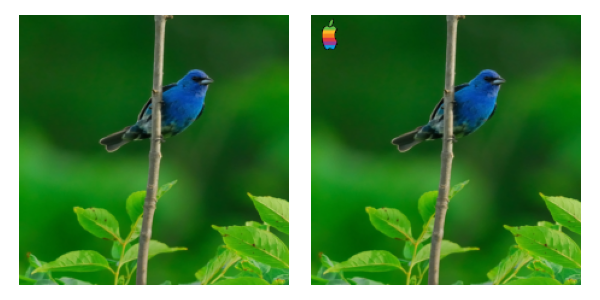
\includegraphics[scale=0.6]{./Slike/imagenet1k_uzorak_badnets.png}
  \caption{Primjer primjene napada BadNets.\ Izvornoj slici (lijevo) dodaje se okidač kako bi nastala zatrovana slika (desno).}
  \label{fig:badnets}
\end{figure}

\pagebreak
  
\subsection{Napad Blend}
\label{sub:blend}

Napad Blend provodi miješanje zadanog okidača sa svakim odabranim ulaznim primjerom.\ Pritom je jačina napada određena hiperparametrom $\alpha$ koji nazivamo jačina miješanja (engl.\ \textit{blending strength}).\ 
Primjenu napada Blend možemo prikazati jednadžbom:

\begin{equation}
  \bm{\tilde{x}} = (1 - \alpha) \cdot \bm{x} + \alpha \cdot \bm{t}
  \label{eq:blend}
\end{equation}

Pri čemu $\bm{x}$ označava ulazni primjer, $\bm{t}$ okidač, a $\bm{\tilde{x}}$ zatrovani primjer.\ Kod napada Blend, izmjene oznaka su uobičajeno tipa \textit{all-to-one}.\

\begin{figure}[h]
  \centering
  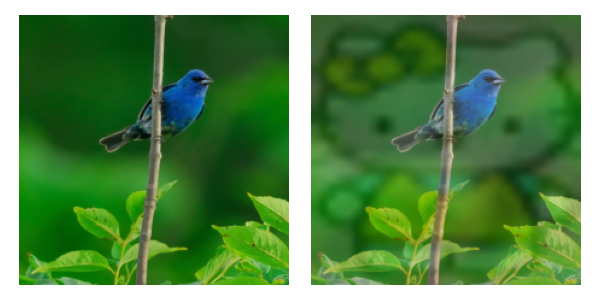
\includegraphics[scale=0.6]{./Slike/imagenet1k_uzorak_blend.png}
  \caption{Primjer primjene napada Blend.\ Izvorna slika (lijevo) miješa se s okidačem uz $\alpha = 0.2$ kako bi nastala zatrovana slika (desno).}
  \label{fig:blend}
\end{figure}
  
\subsection{Napad WaNet}
\label{sub:wanet}

Napad WaNet provodi geometrijsku transformaciju svakog odabranog ulaznog primjera koristeći nasumično generirano deformacijsko polje.\ Deformacijsko polje svakom pikselu odredišne slike dodjeljuje vektor pomaka prema pikselu izvorne slike.\
Pritom hiperparametar $k$ određuje veličinu nasumično generiranog polja šuma na temelju kojeg se skaliranjem i interpolacijom dobiva konačno deformacijsko polje, a hiperparametar $s$ određuje jačinu deformacije.\ 
Primjenu napada WaNet možemo definirati jednadžbom:

\begin{equation}
  \bm{\tilde{x}} = \mathcal{W}(\bm{x}, \bm{M}(k, s))
  \label{eq:wanet}
\end{equation}

\pagebreak

Pri čemu $\bm{x}$ označava ulazni primjer, $\bm{M}$ deformacijsko polje generirano uz hiperparametre $k$ i $s$, $\mathcal{W}$ primjenu deformacijskog polja na ulazni primjer, a $\bm{\tilde{x}}$ zatrovani primjer.\ 
Kao i kod napada Blend, kod napada WaNet su izmjene oznaka uobičajeno tipa \textit{all-to-one}.\ 

\begin{figure}[h]
  \centering
  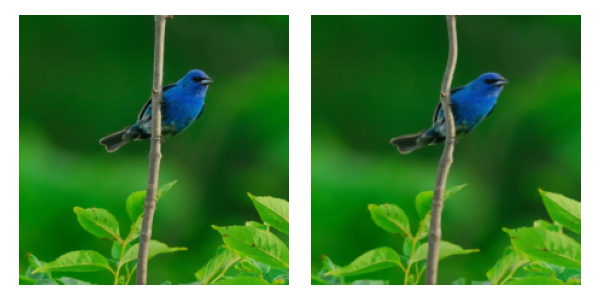
\includegraphics[scale=0.6]{./Slike/imagenet1k_uzorak_wanet.png}
  \caption{Primjer primjene napada WaNet.\ Izvorna slika (lijevo) transformira se koristeći deformacijsko polje uz $k = 8$ i $s = 4$ kako bi nastala zatrovana slika (desno).\ Hiperparametri $k$ i $s$ su uvećani kako bi učinak trovanja bio uočljiviji.}
  \label{fig:wanet}
\end{figure}

\section{Primjeri algoritama za obranu od zatrovanih podataka}
\label{sek:primjeri_obrana_trovanje}

U ovome radu, rezultate okvira VIBE uspoređujemo s rezultatima tri algoritma za obranu od zatrovanih podataka: \textit{Anti-backdoor learning} (ABL)~\cite{li2021anti}, \textit{Decoupling based defense} (DBD)~\cite{huang2022backdoor} te \textit{Adaptively splitting dataset-based defense} (ASD)~\cite{gao2023backdoor}.\

\subsection{Obrana ABL}
\label{sub:abl}

Algoritam \textit{Anti-backdoor learning} (ABL) sastoji se od dva glavna koraka: izoliranje zatrovanih podataka (engl.\ \textit{backdoor isolation}) i odučavanje trovanja (engl. \textit{backdoor unlearning}).\ 
Osnovna ideja ove obrane je da se nakon određenog broja epoha učenja uz posebno definiran gubitak izolira određeni broj primjera za koje se smatra da su zatrovani.\  
Nakon prvog koraka, ti se primjeri koriste za odučavanje trovanja, dok se preostali primjeri koriste za standardno učenje.\ 
  
Konkretno, cilj prvog koraka je zadržati vrijednost gubitka svakog pojedinog primjera oko praga $\gamma$.\
Kako bi ovo postigli, autori predlažu korištenje gradijentnog uspona u slučaju da gubitak primjera padne ispod praga, dok se inače koristi gradijentni spust.\ Gubitak u prvom koraku možemo prikazati jednadžbom:

\begin{equation}
  \mathcal{L}_1 = \mathbb{E}_{(\bm{x}, y) \sim \mathcal{D}} \left[ \operatorname{sign} \left( \ell(f_{\bm{\theta}}(\bm{x}), y) - \gamma \right) \cdot \ell(f_{\bm{\theta}}(\bm{x}), y) \right]
  \label{eq:abl1}
\end{equation}

Pritom $(\bm{x}, y) \sim \mathcal{D}$ označava primjer $\bm{x}$ s pripadnom oznakom $y$ iz skupa podataka $\mathcal{D}$, $f_{\bm{\theta}}(\bm{x})$ izlaz modela parametriziranog parametrima $\bm{\theta}$, $\ell(\hat{y}, y)$ gubitak za predviđenu oznaku $\hat{y}$ i stvarnu oznaku $y$, a $\operatorname{sign}$ operaciju signum.\ 
  
Ideja je da će gubitak za zatrovane primjere veoma brzo pasti ispod praga te će se za njih često aktivirati gradijentni uspon, dok će gubitak čistih primjera sporije padati i stabilizirati se oko praga.\ 
Nakon zadanog broja epoha, izolira se udio $p$ primjera s najnižim gubitkom i proglašava potencijalnim zatrovanim skupom.\ Važno je napomenuti da bismo prvi korak ABL-a mogli zamijeniti proizvoljnim algoritmom detekcije zatrovanih primjera.\ 
  
U drugom koraku, učenje se u svakoj epohi provodi zasebno za procijenjeni čisti odnosno zatrovani skup.\ 
Dok se učenje na čistom skupu provodi uz standardni gradijentni spust, učenje na zatrovanom skupu provodi se uz gradijentni uspon kako bi model odučili od trovanja.\ 
Ovo je moguće zato što je trovanje najčešće realizirano uz samo jedan ciljni razred tj.\ uz \textit{all-to-one} način izmjene oznaka.\ Gubitak u drugom koraku možemo prikazati jednadžbom:

\begin{equation}
  \mathcal{L}_2 = \mathbb{E}_{(\bm{x}, y) \sim \hat{\mathcal{D}}_c} \left[ \ell(f_{\bm{\theta}}(\bm{x}), y) \right] - \mathbb{E}_{(\bm{x}, y) \sim \hat{\mathcal{D}}_b} \left[ \ell(f_{\bm{\theta}}(\bm{x}), y) \right]
  \label{eq:abl2}
\end{equation}

Pritom $\hat{\mathcal{D}}_c$ označava procijenjeni čisti skup, a $\hat{\mathcal{D}}_b$ procijenjeni zatrovani skup.\

\subsection{Obrana DBD}
\label{sub:dbd}

Algoritam \textit{Decoupling based defense} (DBD) problem učenja modela na zatrovanim podatcima razdvaja na tri koraka.\ 
Pritom DBD model tretira kao dvije povezane cjeline: ekstraktor značajki (engl.\ \textit{feature extractor}) te klasifikator (najčešće nekoliko potpuno-povezanih slojeva).\  
Ekstraktor značajki za ulazni primjer na izlazu daje vektor značajki tj.\ ugrađivanje (engl.\ \textit{embedding}) u latentnom metričkom prostoru.\ 
S druge strane, klasifikator za ugrađivanje na ulazu predviđa jednu od mogućih oznaka.\

\begin{figure}[h]
  \centering
  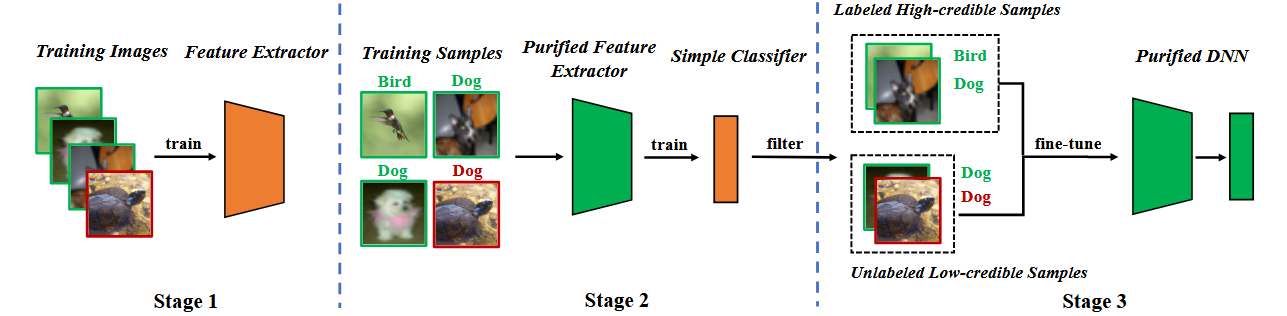
\includegraphics[scale=0.65]{./Slike/dbd.png}
  \caption{Prikaz glavnih koraka obrane DBD.\ Preuzeto iz\cite{huang2022backdoor}}
  \label{fig:dbd}
\end{figure}
  
U prvom koraku, DBD uči ekstraktor značajki koristeći proizvoljan algoritam samonadziranog učenja~\cite{jaiswal2020survey} na slikama bez oznaka.\ 
Pošto algoritmi samonadziranog učenja uobičajeno uključuju korištenje jakih augmentacija ulaznih primjera, kvaliteta okidača kod zatrovanih primjera bit će narušena.\ 
Dodatno, pošto se model u ovoj fazi uči bez oznaka, u prvom koraku nije moguće zatrovati ekstraktor značajki.\ Drugim riječima, na kraju prvog koraka imat ćemo naučen čisti ekstraktor značajki.\ 

U drugom koraku, parametri ekstraktora značajki su zamrznuti, a klasifikator učimo koristeći klasično nadzirano učenje na podatcima s oznakama.\ 
Pritom kao funkciju gubitka koristimo simetričnu unakrsnu entropiju - pokazano je da korištenje iste rezultira višim gubitkom kod zatrovanih primjera~\cite{wang2019symmetric}.\ 
Ipak, ako bismo koristili samo ova dva koraka, dobiveni model ne bi imao performanse jednake stanju tehnike jer smo ekstraktor značajki učili bez oznaka.\ 
Zbog toga, važno je napraviti podjelu skupa podataka na čisti i zatrovani skup te nakon toga ugoditi (engl.\ \textit{fine-tune}) cijeli model.\ 
Kod algoritma DBD, ova podjela se radi na temelju iznosa gubitka: udio $\alpha$ primjera s najnižim iznosom gubitka smatrat ćemo vjerodostojnim tj.\ čistim skupom, dok ćemo preostale primjere smatrati zatrovanima.\ 

Treći korak koristi podjelu na čisti i zatrovani skup kako bi dodatno ugodio parametre cijelog modela.\ 
Konkretno, zatrovanom skupu uklanjamo oznake te potom model učimo koristeći proizvoljni algoritam polu-nadziranog učenja~\cite{van2020survey}.\ 
Na kraju ovog koraka, imat ćemo naučen cjelokupni model otporan na zatrovane primjere.\ 

\pagebreak

\subsection{Obrana ASD}
\label{sub:asd}

Algoritam \textit{Adaptively splitting dataset-based defense} (ASD) problem učenja modela na zatrovanim podatcima razdvaja na tri koraka.\ 
Tijekom sva tri koraka, održavaju se dva skupa podataka: čisti i zagađeni skup.\ Pritom se u čistom skupu nalaze podatci za koje je velika vjerojatnost da su čisti, dok se u zagađenom skupu nalaze zatrovani podatci, kao i preostali čisti podatci.\ 
Kroz učenje, čisti skup se povećava dodavanjem primjera iz zagađenog skupa.\ Konačno, na kraju učenja bi zagađeni skup trebao sadržavati isključivo zatrovane podatke.\ 
Parametri modela uvijek se ažuriraju na temelju proizvoljnog polu-nadziranog gubitka, pri čemu se zagađeni skup koristi za učenje bez oznaka.\   

\begin{figure}[h]
  \centering
  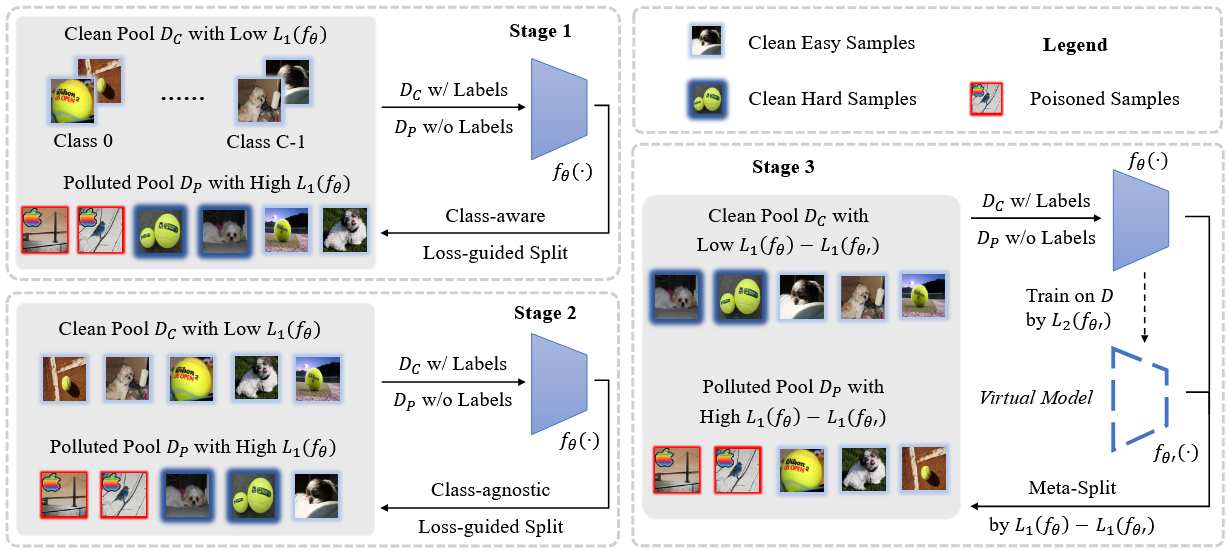
\includegraphics[scale=0.65]{./Slike/asd.png}
  \caption{Prikaz glavnih koraka obrane ASD.\ $D_C$ predstavlja čisti skup, a $D_P$ zagađeni skup.\ Preuzeto iz\cite{gao2023backdoor}}
  \label{fig:asd}
\end{figure}
  
U prvom koraku, čisti skup se inicijalizira na mali broj provjereno čistih primjera (na primjer, po $10$ primjera za svaki razred), dok se zagađeni skup inicijalizira na cijeli skup podataka.\ 
Svakih $t$ epoha učenja, u čisti skup se iz zagađenog skupa dodaje $n$ primjera iz svakog pojedinog razreda koji imaju najniži gubitak $\mathcal{L}_1$.\ Pritom kao funkciju gubitka $\mathcal{L}_1$ koristimo simetričnu unakrsnu entropiju kako bi zatrovani primjeri imali što viši gubitak.\ 
Ovu podjelu zovemo razredno-svjesna podjela vođena gubitkom (engl.\ \textit{class-aware loss-guided split}).\ 
  
Tijekom drugog koraka, čisti skup značajno proširujemo dodavanjem udjela $\alpha$ zagađenog skupa.\ 
Pritom se dodaju primjeri iz cijelog skupa (neovisno o razredu) koji imaju najniži gubitak $\mathcal{L}_1$.\ 
Ovu podjelu zovemo razredno-nesvjesna podjela vođena gubitkom (engl.\ \textit{class-agnostic loss-guided split}).\ 
  
Nakon prva dva koraka ASD-a, u zagađenom skupu preostaju zatrovani primjeri, ali i neki teški primjeri specifični za model.\ 
Zbog toga što model nismo učili na teškim primjerima s oznakama, performanse modela trenutno su niže od stanja tehnike.\ Kako bismo dodali i teške primjere u čisti skup, svaku epohu trećeg koraka konstruiramo virtualni model.\ 
Virtualni model inicijaliziramo parametrima glavnog modela te potom provodimo jednu epohu nadziranog učenja na zagađenom skupu uz korištenje gubitka $\mathcal{L}_2$.\ Kao funkciju gubitka $\mathcal{L}_2$ koristimo standardnu unakrsnu entropiju.\ 
Nakon učenja virtualnog modela, mjerimo smanjenje gubitka definirano jednadžbom:

\begin{equation}
  \Delta \mathcal{L} = \mathcal{L}_1(f_{\bm{\theta}}) - \mathcal{L}_1(f_{\bm{\theta'}})
  \label{eq:asd}
\end{equation}

Pritom $f_{\bm{\theta}}$ označava glavni model parametriziran parametrima $\bm{\theta}$, a $f_{\bm{\theta'}}$ predstavlja virtualni model parametriziran parametrima $\bm{\theta'}$ dobivenim nakon jedne epohe nadziranog učenja na zagađenom skupu.\ 
Konačno, udio $\gamma$ primjera s najmanjim smanjenjem gubitka dodajemo u čisti skup.\ Intuicija iza ove podjele je da su zatrovani podatci lagani za naučiti, tako da već nakon jedne epohe nadziranog učenja isti imaju veoma nizak gubitak, dok teški čisti primjeri i dalje imaju visok gubitak.\ 
Važno je napomenuti da se virtualni model koristi isključivo za provođenje podjele na temelju smanjenja gubitka.\ 
Ovu podjelu zovemo meta-podjela (engl.\ \textit{meta-split}) jer je pristup s učenjem virtualnog modela inspiriran područjem meta-učenja (engl.\ \textit{meta-learning})~\cite{vilalta2002perspective}.\
Na kraju trećeg koraka, u čistom skupu će se nalaziti gotovo svi čisti primjeri, a dobiveni model će imati izvrsne performanse uz otpornost na zatrovane primjere.\

%-------------------------------------------------------------------------------
\chapter{Problem zašumljenih oznaka}
\label{pog:zasumljeni}

\section{Primjeri metoda zašumljivanja oznaka}
\label{sek:primjeri_zasumljivanja}

\section{Primjeri algoritama za učenje na zašumljenim oznakama}
\label{sek:primjeri_obrana_zasumljivanje}
%-------------------------------------------------------------------------------
\chapter{Samonadzirano učenje}
\label{pog:samonadzirano}


%-------------------------------------------------------------------------------
\chapter{Algoritam maksimizacije očekivanja}
\label{pog:em_algoritam}


%-------------------------------------------------------------------------------
\chapter{Transportni problem}
\label{pog:transport}


%-------------------------------------------------------------------------------
\chapter{VIBE}
\label{pog:vibe}


%-------------------------------------------------------------------------------
\chapter{Skup podataka}
\label{pog:skup}


%-------------------------------------------------------------------------------
\chapter{Eksperimenti}
\label{pog:eksperimenti}


%--- ZAKLJUČAK / CONCLUSION ----------------------------------------------------
\chapter{Zaključak}
\label{pog:zakljucak}


%--- LITERATURA / REFERENCES ---------------------------------------------------

% Literatura se automatski generira iz zadane .bib datoteke / References are automatically generated from the supplied .bib file
% Upiši ime BibTeX datoteke bez .bib nastavka / Enter the name of the BibTeX file without .bib extension
\bibliography{literatura}


%--- SAŽETAK / ABSTRACT --------------------------------------------------------

% Sažetak na hrvatskom
\begin{sazetak}
  Sažetak...
\end{sazetak}

\begin{kljucnerijeci}
  prva ključna riječ; druga ključna riječ; treća ključna riječ
\end{kljucnerijeci}


\end{document}
